\section{Evaluation}
\label{sec:Eval}

\subsection{Program Synthesis}

\subsection{Parameterized Hash Functions}

We simulated the voting algorithm of the previous section by treating all of the
numbers in the ranges of $[0, 2^{8}]$ and $[0, 2^{16}]$ as memory addresses and
hashing them against a simple array of 4 caches of sizes 3, 2, 2, and 1.  While
we tested mainly with this setup, the number of caches and their sizes are
widely configurable.  The graphs below show the histograms of the homed data,
namely, the number of addresses in the space that were mapped to the given
cache.  Ideally, we expect the number of addresses in each cache to follow the
3, 2, 2, 1 distribution.  The metrics chosen were the modulo scheme, which is
identical to the scheme that chooses the distinguished cache and which hashes
the memory address and modulos by the number of caches, the sum of positive
bits, and addition of the median number of caches.


\begin{figure}[h]
  \centering
  \begin{minipage}[b]{0.4\textwidth}
    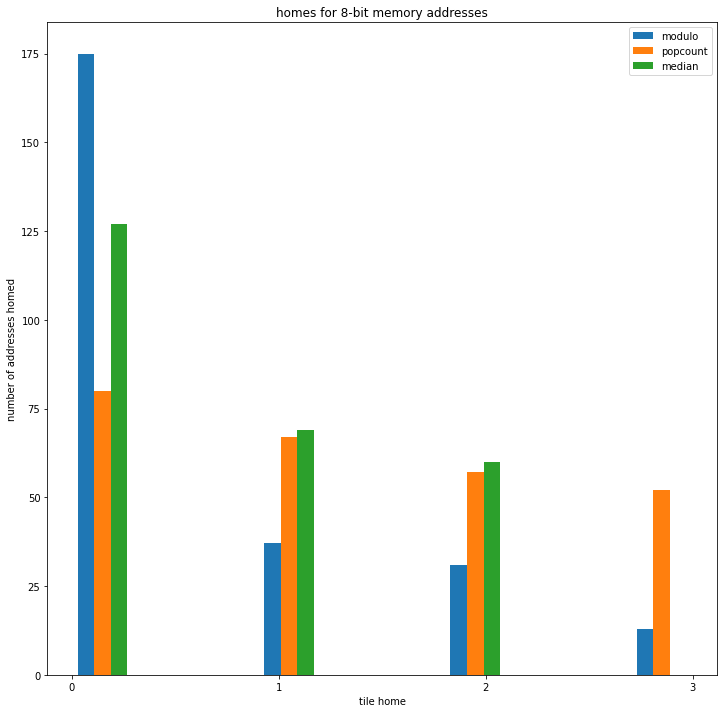
\includegraphics[width=\textwidth]{homes.png}
    \caption{256 bit memory space}
    \label{Fig:homes}
  \end{minipage}
  \hfill
  \begin{minipage}[b]{0.4\textwidth}
    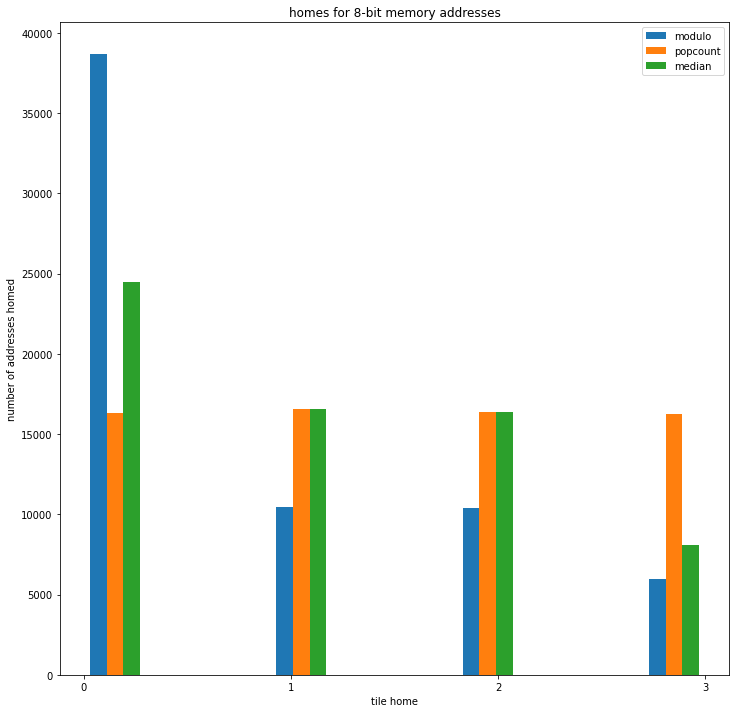
\includegraphics[width=\textwidth]{homes2.png}
    \caption{65536 bit memory space }
    \label{Fig:homes2}
  \end{minipage}
\end{figure}

From the graphs we can see first that popcount is not a good metric for deciding
homes as it collapses to the uniform distribution with enough data.
Interestingly, the remaining two approaches, modulo and median, do roughly match
the distribution of cache sizes, with most data going to the default largest
cache, less going to the middle two largest caches, and the least going to the
smallest cache.  The median performs much closer however it is not clear what
this intuitively captures about the data.  Finally, the modulo scheme seems to
unduly weight the largest cache.  While thse don't quite capture the
distribution, it is clear that they can be modified to provide a more robust
picture of the cache size distributions.  

There are a number of improvements that we could make as a second pass in
hardening this approach.  The number and sizes of caches should be changed
widely, and specifically, the sizes of the caches should be powers of 2, or
simply arithmetic combinations of powers of 2, to mimic real world
conditions. Additionally, as noted previously, the weighting function is crucial
to observing a smooth distribution matching the cache sizes.  The options we
tried should be expanded to find better matches.

Finally, the hash function we used was the Pearson function, which is
traditionally based on a 256-bit table of randomized seed values.  To minimize
the impact of this on a production many-core system, this can be replaced with
alternative metrics, such as a subtraction of the memory address from
256.Ultimately, however, the scheme is a flexible and highly configurable
approach to parameterizing the usual hash functions used for hardware, and we
look forward to elaborating on the idea.  
